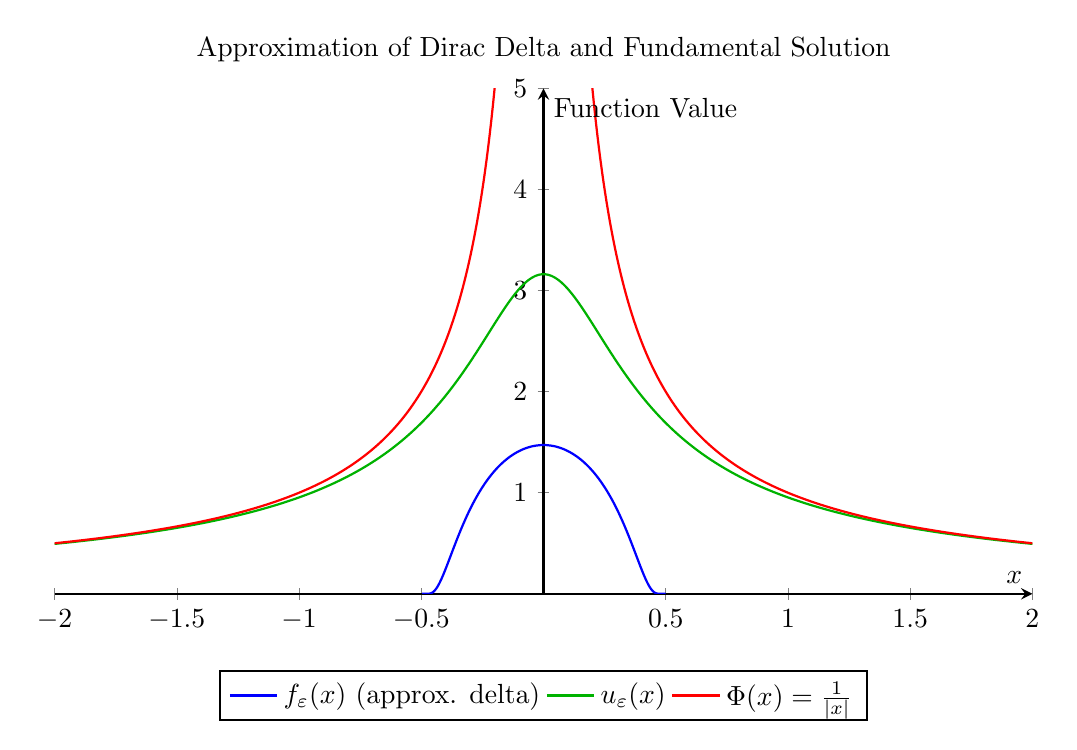
\begin{tikzpicture}
\begin{axis}[
    title={Approximation of Dirac Delta and Fundamental Solution},
    axis lines=middle,
    xlabel={$x$},
    ylabel={Function Value},
    legend style={at={(0.5,-0.15)}, anchor=north, legend columns=3},
    xmin=-2, xmax=2,
    ymin=0, ymax=5,
    samples=300,
    domain=-2:2,
    width=14cm,
    height=8cm,
    thick,
]

% Mollifier f_epsilon (bump function)
\addplot[blue, thick, domain=-0.5:0.5] {4 * exp(-1/(1 - (x/0.5)^2))};
\addlegendentry{$f_\varepsilon(x)$ (approx. delta)}

% Solution u_epsilon (smoothed 1/|x| version)
\addplot[green!70!black, thick, domain=-2:2] {1 / sqrt(x^2 + 0.1)};
\addlegendentry{$u_\varepsilon(x)$}

% Fundamental solution 1/|x|
\addplot[red, thick, domain=0.05:2] {1/x};
\addplot[red, thick, domain=-2:-0.05] {-1/x}; % Symmetric for absolute value
\addlegendentry{$\Phi(x) = \frac{1}{|x|}$}

\end{axis}
\end{tikzpicture}